\documentclass[10pt]{beamer}
\usepackage{amsmath,amsthm,amssymb}
\usepackage{mathtext}
\usepackage[T1,T2A]{fontenc}
\usepackage[utf8]{inputenc}
\usepackage[english,russian]{babel}
\usepackage{colortbl}
\usepackage{blindtext}
\usepackage{listings}
\usetheme{default}
\usecolortheme[named=black]{structure}
\newenvironment{comment}{}{}
\title{\textcolor{black}{\LARGE \textbf{Анализ алгоритмов обучения нейронных сетей на примере решения задачи распознавания рукописных цифр}}}

%\author{ Докладчик \\ \textbf{Глазов Николай Григорьевич}}

\author{ 
 \hfill\hbox to\maxl{группа:  МКЗ-430127к\hfill}\\
 \hfill\hbox to\maxl{Глазов Н.Г. \hfill}\\
 \hfill\hbox to\maxl{Научный руководитель:\hfill}\\
 \hfill\hbox to\maxl{к.ф.-м.н\hfill}\\
 \hfill\hbox to\maxl{Горбенко А. А.\hfill}}
\date{2017}
\begin{document}
%1%%%%%%%%%%%%%%%%%%%%%%%%%%%%%%%%
\begin{frame}

\makebox[0.35\paperwidth][t]{
\includegraphics[width=4cm]{1.eps} \hfill}
 {\global\arrayrulewidth=0.5mm}
  \arrayrulecolor{red}\hline
  
  %\setbeamercolor{coloredboxstuff}{fg=black,bg=black!10!gray}
  %\begin{beamercolorbox}[wd=1\textwidth,sep=1em]{coloredboxstuff}
  \titlepage
  %\end{beamercolorbox}
\noalign
\end{frame}

%2%%%%%%%%%%%%%%%%%%%%%%%%%%%%%%%%
\begin{frame}\frametitle{\makebox[0.15\paperwidth][t]{
\includegraphics[width=4cm]{1.eps}
\parbox[#1]{.433\textwidth}{\centering \textcolor{black}{ {\small{Анализ алгоритмов обучения.}}}}
\parbox[#1]{.233\textwidth}{\raggedleft\textcolor{black}{\small {Глазов Н. Г.}}}\par\smallskip%
}
 {\global\arrayrulewidth=0.5mm}
  \arrayrulecolor{red}\hline
  \LARGE{Актуальность работы}
  }
  \LARGE{
  \begin{itemize}
      \item Градиентный спуск
      \item Методы оптимизации в библиотеках нейронных сетей(Keras, Caffe)
      \item Сравнение эффективности  методов
  \end{itemize}
  }  
\end{frame}

%3%%%%%%%%%%%%%%%%%%%%%%%%%%%%%%%%
\begin{frame}\frametitle{\makebox[0.15\paperwidth][t]{
\includegraphics[width=4cm]{1.eps}
\parbox[#1]{.433\textwidth}{\centering \textcolor{black}{ {\small{Анализ алгоритмов обучения.}}}}
\parbox[#1]{.233\textwidth}{\raggedleft\textcolor{black}{\small {Глазов Н. Г.}}}\par\smallskip%
}
 {\global\arrayrulewidth=0.5mm}
  \arrayrulecolor{red}\hline
  \Large{
    Задача распознавания рукописных цифр}} 
\Large{
    Пример изображения:
\begin{figure}[b]
    \centering
    \includegraphics[width=0.4\textwidth]{13931_6.eps}
    \caption{Изображение рукописной цифры 6.}
    \label{fig:13931_6}
\end{figure}
}  
\end{frame}

%5%%%%%%%%%%%%%%%%%%%%%%%%%%%%%%%%
\begin{frame}\frametitle{\makebox[0.15\paperwidth][t]{
\includegraphics[width=4cm]{1.eps}
\parbox[#1]{.433\textwidth}{\centering \textcolor{black}{ {\small{Анализ алгоритмов обучения.}}}}
\parbox[#1]{.233\textwidth}{\raggedleft\textcolor{black}{\small {Глазов Н. Г.}}}\par\smallskip%
}
 {\global\arrayrulewidth=0.5mm}
  \arrayrulecolor{red}\hline
  \Large{Нейронные сети}
  } 
\Large{
    \begin{itemize}
        \item Адаптивность. 
        \item Масштабируемость.
        \item Параллельная обработка информации.
        \item Запоминание контекстной информации. 
    \end{itemize}
}
  
\end{frame}

%4%%%%%%%%%%%%%%%%%%%%%%%%%%%%%%%%
\begin{frame}\frametitle{\makebox[0.15\paperwidth][t]{
\includegraphics[width=4cm]{1.eps}
\parbox[#1]{.433\textwidth}{\centering \textcolor{black}{ {\small{Анализ алгоритмов обучения.}}}}
\parbox[#1]{.233\textwidth}{\raggedleft\textcolor{black}{\small {Глазов Н. Г.}}}\par\smallskip%
}
 {\global\arrayrulewidth=0.5mm}
  \arrayrulecolor{red}\hline
  \LARGE{Цель работы}
  } 
\Large{
Сравнительное исследование и анализ эффективности различных методов оптимизации при обучении нейронных сетей для решения задачи распознавания рукописных арабских цифр
}
  
\end{frame}

%6%%%%%%%%%%%%%%%%%%%%%%%%%%%%%%%%

\begin{frame}\frametitle{\makebox[0.15\paperwidth][t]{
\includegraphics[width=4cm]{1.eps}
\parbox[#1]{.433\textwidth}{\centering \textcolor{black}{ {\small{Анализ алгоритмов обучения.}}}}
\parbox[#1]{.233\textwidth}{\raggedleft\textcolor{black}{\small {Глазов Н. Г.}}}\par\smallskip%
}
 {\global\arrayrulewidth=0.5mm}
  \arrayrulecolor{red}\hline
  \Large{Рассмотрены в работе}
  }  
\Large{
    \begin{itemize}
        \item Однослойный персептрон Розенблатта. 
        \item Многослойные нейронные сети.
    \end{itemize}
} 
\end{frame}

%7%%%%%%%%%%%%%%%%%%%%%%%%%%%%%%%%

\begin{frame}\frametitle{\makebox[0.15\paperwidth][t]{
\includegraphics[width=4cm]{1.eps}
\parbox[#1]{.433\textwidth}{\centering \textcolor{black}{ {\small{Анализ алгоритмов обучения.}}}}
\parbox[#1]{.233\textwidth}{\raggedleft\textcolor{black}{\small {Глазов Н. Г.}}}\par\smallskip%
}
 {\global\arrayrulewidth=0.5mm}
  \arrayrulecolor{red}\hline
  \Large{
    Методы оптимизации}
  } 
\Large{
\begin{itemize}
    \item Метод стохастического градиента с инерцией(Nesterov Accelerated Gradient).
    \item Метод адаптивного градиента (Adagrad).
    \item Метод адаптивного скользящего среднего градиентов (RMSProp).
    \item Метод адаптивного шага обучения(Adadelta).
    \item Метод адаптивной инерции (Adam).
\end{itemize}
}
  
\end{frame}

%8%%%%%%%%%%%%%%%%%%%%%%%%%%%%%%%%

\begin{frame}\frametitle{\makebox[0.15\paperwidth][t]{
\includegraphics[width=4cm]{1.eps}
\parbox[#1]{.433\textwidth}{\centering \textcolor{black}{ {\small{Анализ алгоритмов обучения.}}}}
\parbox[#1]{.233\textwidth}{\raggedleft\textcolor{black}{\small {Глазов Н. Г.}}}\par\smallskip%
}
 {\global\arrayrulewidth=0.5mm}
  \arrayrulecolor{red}\hline
  \Large{
    Метод адаптивного градиента (Adagrad).}
  } 
\Large{

Формула пересчёта:
\[g_{t+1} = g_t + \nabla f(w_t)^2 \]
\[w_{t+1} = w_t - \frac{\mu \nabla f(w_t) }{\sqrt{g_{t+1} + \epsilon)} }  \] 

Используем предыдущие приращения градиента, чтобы редким, но важным признакам давать больший вес.
}
  
\end{frame}

%9%%%%%%%%%%%%%%%%%%%%%%%%%%%%%%%%

\begin{frame}\frametitle{\makebox[0.15\paperwidth][t]{
\includegraphics[width=4cm]{1.eps}
\parbox[#1]{.433\textwidth}{\centering \textcolor{black}{ {\small{Анализ алгоритмов обучения.}}}}
\parbox[#1]{.233\textwidth}{\raggedleft\textcolor{black}{\small {Глазов Н. Г.}}}\par\smallskip%
}
 {\global\arrayrulewidth=0.5mm}
  \arrayrulecolor{red}\hline
  \Large{Вычислительный эксперимент}
  } 
\Large{
    \begin{itemize}
    \item Язык Python 2.7.11
    \item Тестовые данные с открытой площадки для соревнований по машинному обучению kaggle.com "Digit Recognizer"
    \item 42000 размеченных чёрно-белых изображений 26*26 пикселей
    \item Обучение на 30 000 примерах
    \item Тестирование на 1 000 примерах
    \end{itemize}
}
  
\end{frame}

%10%%%%%%%%%%%%%%%%%%%%%%%%%%%%%%%%

\begin{frame}\frametitle{\makebox[0.15\paperwidth][t]{
\includegraphics[width=4cm]{1.eps}
\parbox[#1]{.433\textwidth}{\centering \textcolor{black}{ {\small{Анализ алгоритмов обучения.}}}}
\parbox[#1]{.233\textwidth}{\raggedleft\textcolor{black}{\small {Глазов Н. Г.}}}\par\smallskip%
}
 {\global\arrayrulewidth=0.5mm}
  \arrayrulecolor{red}\hline
  \Large{Результаты}
  } 
\Large{
\begin{center}
\arrayrulecolor{black}
  \begin{tabular}{ | l | c | r |}
    % {\global\arrayrulewidth=0.5mm}
  \arrayrulecolor{black}
    \hline
    Метод & Время(сек.) & Точность \\ \hline
    SGD & 52.3 & 89.9\% \\ \hline
    Nesterov & 74.0 & 91.2\% \\ \hline
    Adagrad & 89.3 & 94.0\% \\ \hline
    RMSProp & 92.3 & 84.3\% \\ \hline
    Adadelta & 136.9 & 86.4\% \\ \hline
    Adam & 176.0 & 87.2\% \\
    \hline
  \end{tabular}
\end{center}

}
  
\end{frame}


%11%%%%%%%%%%%%%%%%%%%%%%%%%%%%%%%%

\begin{frame}\frametitle{\makebox[0.15\paperwidth][t]{
\includegraphics[width=4cm]{1.eps}
\parbox[#1]{.433\textwidth}{\centering \textcolor{black}{ {\small{Анализ алгоритмов обучения.}}}}
\parbox[#1]{.233\textwidth}{\raggedleft\textcolor{black}{\small {Глазов Н. Г.}}}\par\smallskip%
}
 {\global\arrayrulewidth=0.5mm}
  \arrayrulecolor{red}\hline
  \Large{Процесс обучения для метода стохастического градиента с инерцией}
  } 
\Large{
\begin{figure}[b]
    \centering
    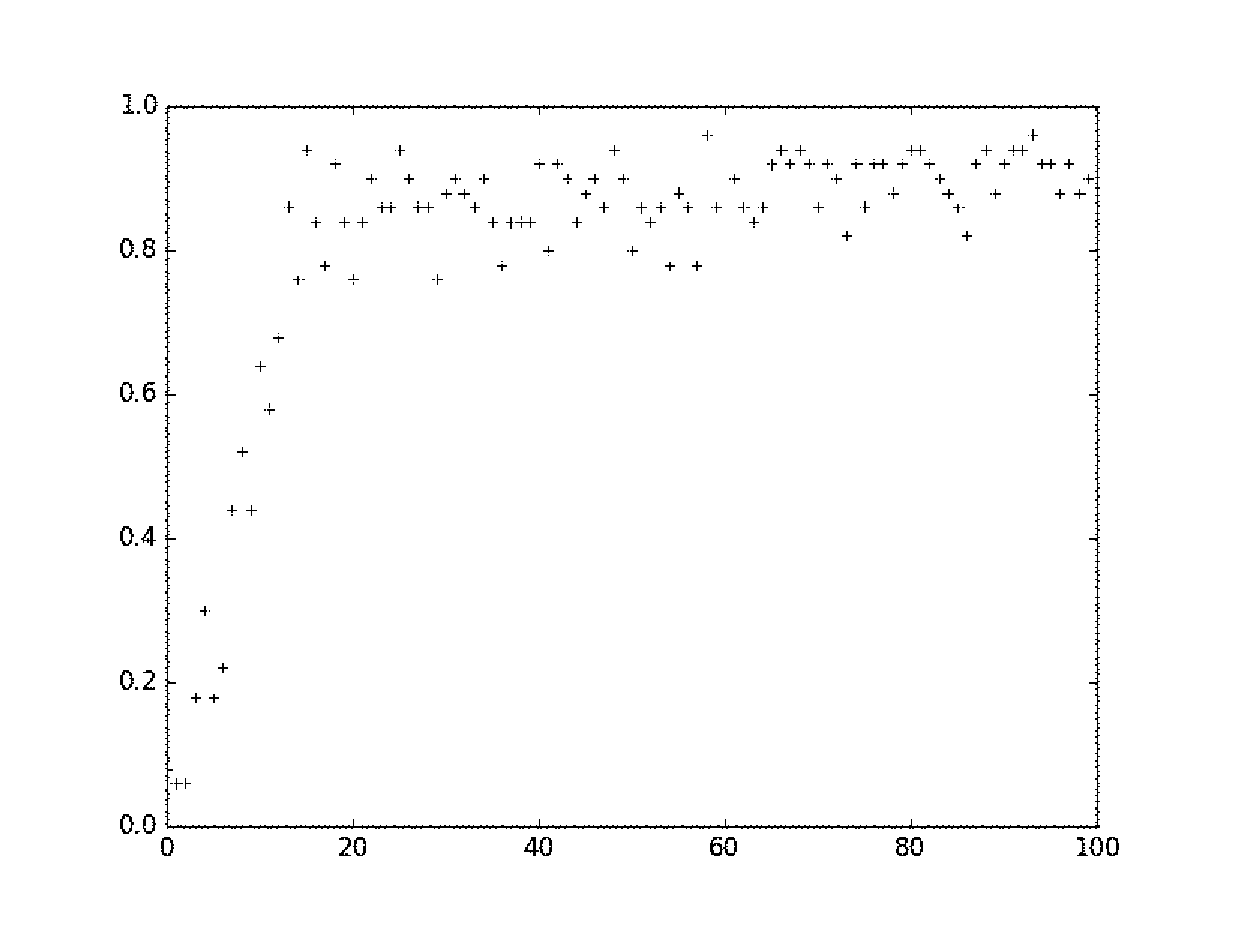
\includegraphics[width=0.7\textwidth]{Nesterov.eps}
    %\caption{Метод стохастического градиента с инерцией(Nesterov Accelerated Gradient).}
    \label{fig:nesterov}
\end{figure}
}
  
\end{frame}


%12%%%%%%%%%%%%%%%%%%%%%%%%%%%%%%%%
\begin{frame}\frametitle{\makebox[0.15\paperwidth][t]{
\includegraphics[width=4cm]{1.eps}
\parbox[#1]{.433\textwidth}{\centering \textcolor{black}{ {\small{Анализ алгоритмов обучения.}}}}
\parbox[#1]{.233\textwidth}{\raggedleft\textcolor{black}{\small {Глазов Н. Г.}}}\par\smallskip%
}
 {\global\arrayrulewidth=0.5mm}
  \arrayrulecolor{red}\hline
  \Large{Процесс обучения для метода адаптивного шага обучения}
  } 
\Large{
\begin{figure}[b]
    \centering
    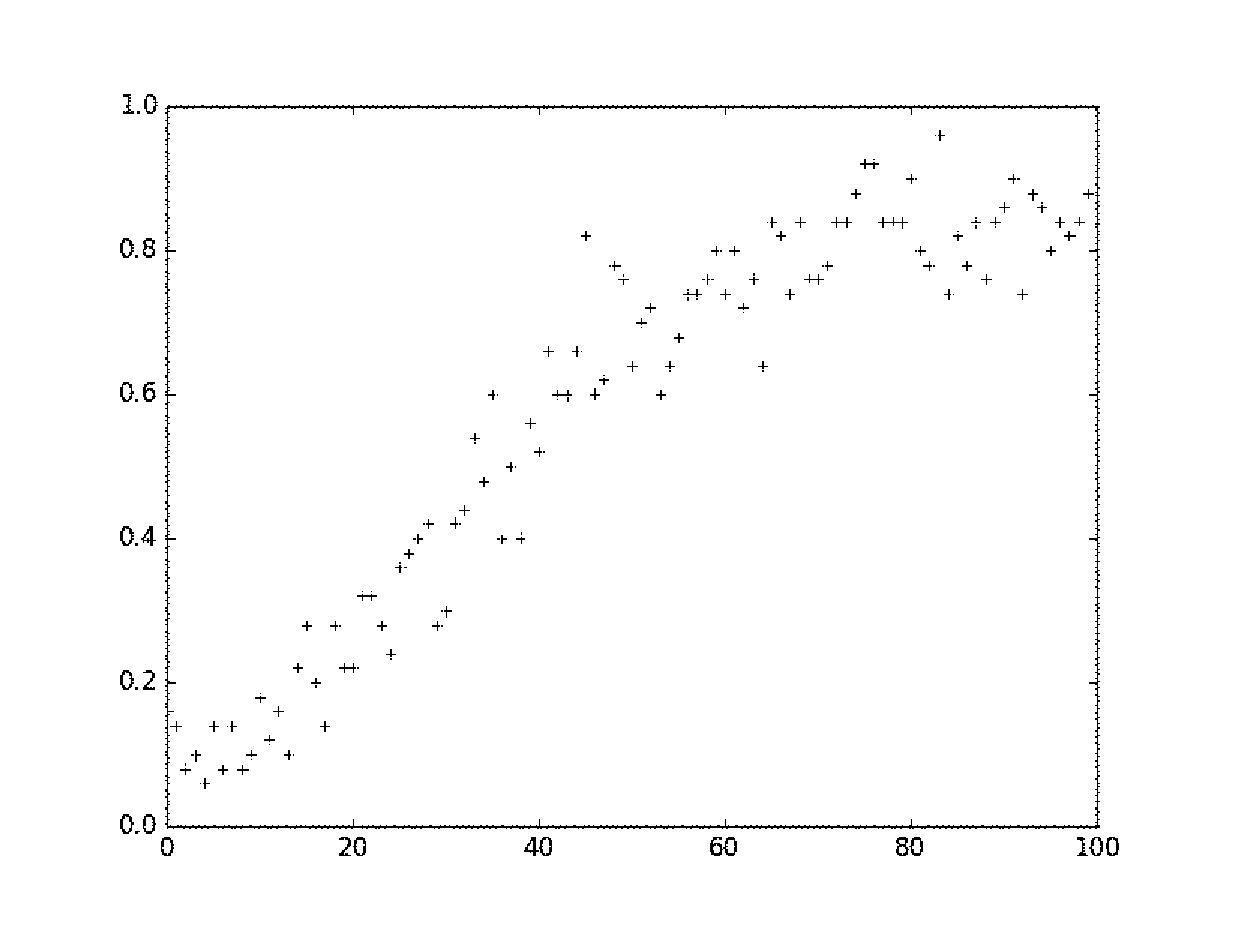
\includegraphics[width=0.7\textwidth]{Adadelta.eps}
    %\caption{Метод стохастического градиента с инерцией(Nesterov Accelerated Gradient).}
    \label{fig:nesterov}
\end{figure}
}
  
\end{frame}



%13%%%%%%%%%%%%%%%%%%%%%%%%%%%%%%%%
\begin{frame}\frametitle{\makebox[0.15\paperwidth][t]{
\includegraphics[width=4cm]{1.eps}
\parbox[#1]{.433\textwidth}{\centering \textcolor{black}{ {\small{Анализ алгоритмов обучения.}}}}
\parbox[#1]{.233\textwidth}{\raggedleft\textcolor{black}{\small {Глазов Н. Г.}}}\par\smallskip%
}
 {\global\arrayrulewidth=0.5mm}
  \arrayrulecolor{red}\hline
  \Large{Процесс обучения для метода адаптивного градиента}
  } 
\Large{
\begin{figure}[b]
    \centering
    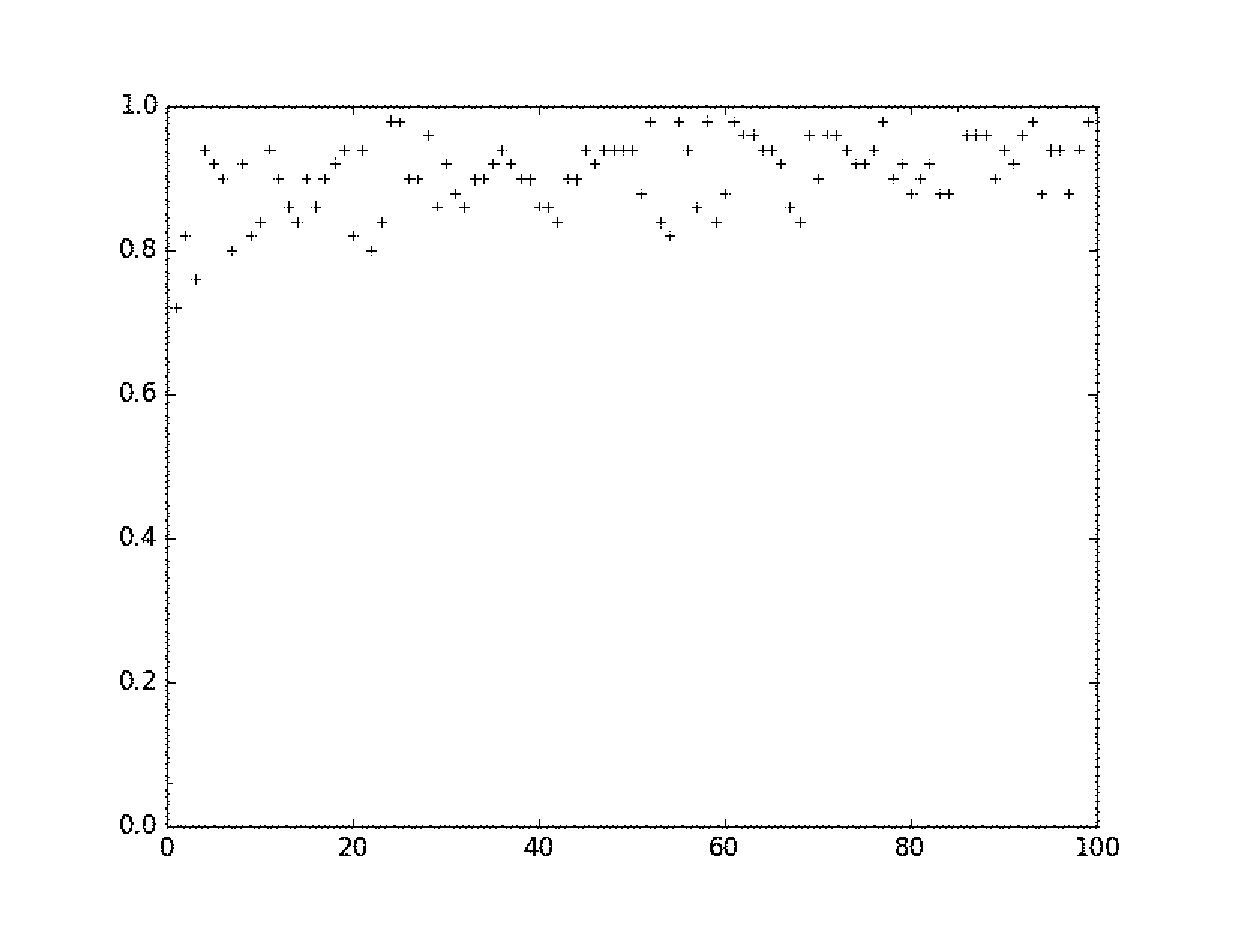
\includegraphics[width=0.7\textwidth]{Adagrad.eps}
    %\caption{Метод стохастического градиента с инерцией(Nesterov Accelerated Gradient).}
    \label{fig:nesterov}
\end{figure}
}
  
\end{frame}

%10%%%%%%%%%%%%%%%%%%%%%%%%%%%%%%%%

\begin{frame}\frametitle{\makebox[0.15\paperwidth][t]{
\includegraphics[width=4cm]{1.eps}
\parbox[#1]{.433\textwidth}{\centering \textcolor{black}{ {\small{Анализ алгоритмов обучения.}}}}
\parbox[#1]{.233\textwidth}{\raggedleft\textcolor{black}{\small {Глазов Н. Г.}}}\par\smallskip%
}
 {\global\arrayrulewidth=0.5mm}
  \arrayrulecolor{red}\hline\LARGE{
Выводы
}} 
\Large{
\begin{itemize}
    \item Средний показатель точности - 90\%
    \item Наилучший результат по точности показал метод адаптивного градиента (Adagrad)
    \item Наилучший результат по времени показал метод стохастического градиента (SGD)
    \item Наиболее эффективным по соотношению точность/время является метод стохастического градиента (SGD)
\end{itemize}
}
  
\end{frame}

% All of the following is optional and typically not needed. 
\appendix
\section<presentation>*{\appendixname}
\subsection<presentation>*{Библиография}

\begin{frame}[allowframebreaks]
  \frametitle<presentation>{Библиография}
    
  \begin{thebibliography}{10}
    
  \beamertemplatebookbibitems
  % Start with overview books.

  \bibitem{Author1990}
    A.~Author.
    \newblock {\em Handbook of Everything}.
    \newblock Some Press, 1990.
 
    
  \beamertemplatearticlebibitems
  % Followed by interesting articles. Keep the list short. 

\addcontentsline{toc}{chapter}{\tocsecindent{Литература}}

\bibitem{bib:keras}
Keras - Deep Learning library
\href{https://keras.io/}{https://keras.io/}

\bibitem{bib:caffe}
Caffe - deep learning framework
\href{http://caffe.berkeleyvision.org/}{http://caffe.berkeleyvision.org/}

\bibitem {hykin:nn} С. Хайкин
\emph{Нейронные сети. Полный курс.}// Издательский дом "Вильямс"\ , 2006

\bibitem{bib:nesterov}
A. Botev, G. Lever, D. Barber Nesterov’s Accelerated Gradient and Momentum as approximations to Regularised Update Descent. // Department of Computer Science University College London. 2016
\bibitem{bib:Adagrad}
J. Duchi, E. Hazan, Y. Singer
Adaptive Subgradient Methods for Online Learning and Stochastic Optimization.//  Journal of Machine Learning Research 12 (2011) 2121-2159 Submitted 3/10; Revised 3/11; Published 7/11
\bibitem{bib:adadelta}
Matthew D. Zeiler Adadelta: an adaptive learning rate method.// Google Inc., USA 2New York University, USA. 2012
\bibitem{bib:adam}
D. P. Kingma, J. L. Ba Adam: a method for stochastic optimization.// Published as a conference paper at ICLR 2015
\bibitem{bib:overview}
An overview of gradient descent optimization algorithms
\href{http://sebastianruder.com/optimizing-gradient-descent/ 2016}{http://sebastianruder.com/optimizing-gradient-descent/ 2016}

\bibitem{bib:rmsprop}
G. Hinton Lecture 6e of his Coursera Class.
\href{"http://www.cs.toronto.edu/tijmen/csc321/slides/lecture_slides_lec6.pdf"}{http://www.cs.toronto.edu/~tijmen/csc321/slides/lecture\_slides\_lec6.pdf}

\bibitem {numpy:package} http://www.numpy.org/
\emph{NumPy is the fundamental package for scientific computing with Python.}

\bibitem {kaggle:com} https://www.kaggle.com
\emph{Digit Recognizer}


  \end{thebibliography}
\end{frame}

\end{document}


